%%%%%%%%%%%%%%%%%%%%%%%%%%%%%%%%%%%%%%%%%
% University/School Laboratory Report
% LaTeX Template
% Version 3.1 (25/3/14)
%
% This template has been downloaded from:
% http://www.LaTeXTemplates.com
%
% Original author:
% Linux and Unix Users Group at Virginia Tech Wiki 
% (https://vtluug.org/wiki/Example_LaTeX_chem_lab_report)
%
% License:
% CC BY-NC-SA 3.0 (http://creativecommons.org/licenses/by-nc-sa/3.0/)
%
%%%%%%%%%%%%%%%%%%%%%%%%%%%%%%%%%%%%%%%%%

%----------------------------------------------------------------------------------------
%	PACKAGES AND DOCUMENT CONFIGURATIONS
%----------------------------------------------------------------------------------------

\documentclass{article}

\usepackage[version=3]{mhchem} % Package for chemical equation typesetting
\usepackage{siunitx} % Provides the \SI{}{} and \si{} command for typesetting SI units
\usepackage{graphicx} % Required for the inclusion of images
\usepackage{natbib} % Required to change bibliography style to APA
\usepackage{amsmath} % Required for some math elements 
\usepackage{enumitem}

\setlength\parindent{0pt} % Removes all indentation from paragraphs

\renewcommand{\labelenumi}{\alph{enumi}.} % Make numbering in the enumerate environment by letter rather than number (e.g. section 6)

%\usepackage{times} % Uncomment to use the Times New Roman font

%----------------------------------------------------------------------------------------
%	DOCUMENT INFORMATION
%----------------------------------------------------------------------------------------

\title{Tutorial 1\\ X Ray Diffraction \\ } % Title

\author{Linda \textsc{Crandall} and Maggie \textsc{Huff}} % Author name

\date{\today} % Date for the report

\begin{document}

\maketitle % Insert the title, author and date

\begin{center}
\begin{tabular}{l r}
Date Performed: & July 7, 2017 \\ % Date the experiment was performed
Instructor: & Chris Pratt % Instructor/supervisor
\end{tabular}
\end{center}

% If you wish to include an abstract, uncomment the lines below
% \begin{abstract}
% Abstract text
% \end{abstract}

%----------------------------------------------------------------------------------------
%	SECTION 1
%----------------------------------------------------------------------------------------

\section{Objective}

To get to know the diffractometer and X'Pert Data Collector, learn how to identify an unknown sample with X'Pert High Score software. 
%(as defined in \ref{definitions}):

%\begin{center}\ce{2 Mg + O2 -> 2 MgO}\end{center}

% If you have more than one objective, uncomment the below:
%\begin{description}
%\item[First Objective] \hfill \\
%Objective 1 text
%\item[Second Objective] \hfill \\
%Objective 2 text
%\end{description}


\section{Results and Conclusions}

Our `unidentified' sample is silicon, which we ascertained after using the search peaks tool in the software. We eliminated the K$\alpha_2$ peaks, as well as peaks whose low intensity categorizes them as background. The program matches the peak pattern to ICDD known peak patterns and returns a match along with a score for how certain the match is.  

\begin{figure}[h]
\begin{center}
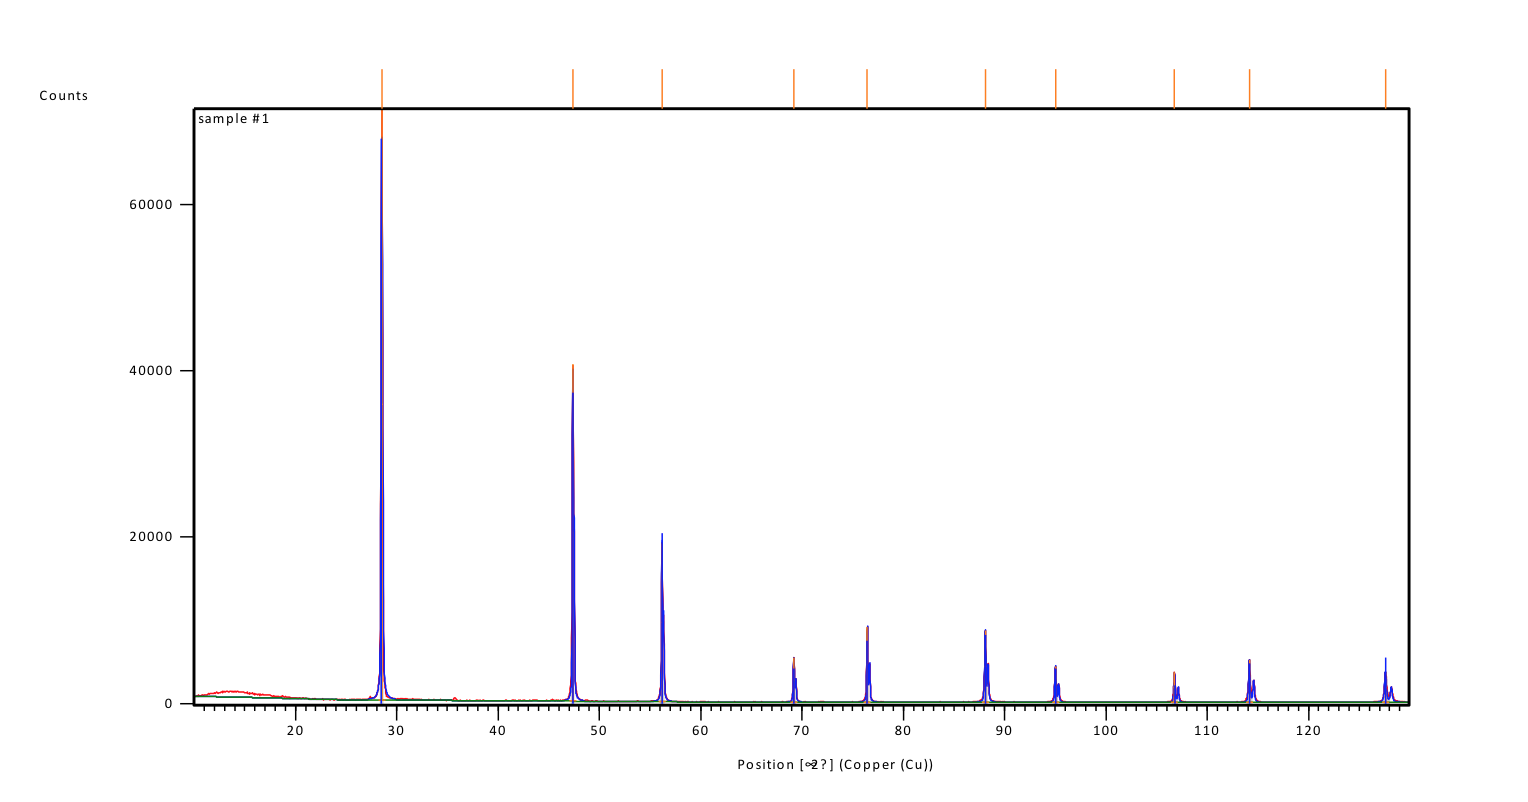
\includegraphics[width=0.65\textwidth]{peaks} % Include the image peaks.png
\caption{background cleaned peaks for sample overlaid with ICDD silicon peaks }
\end{center}
\end{figure}

\begin{figure}[h]
\begin{center}
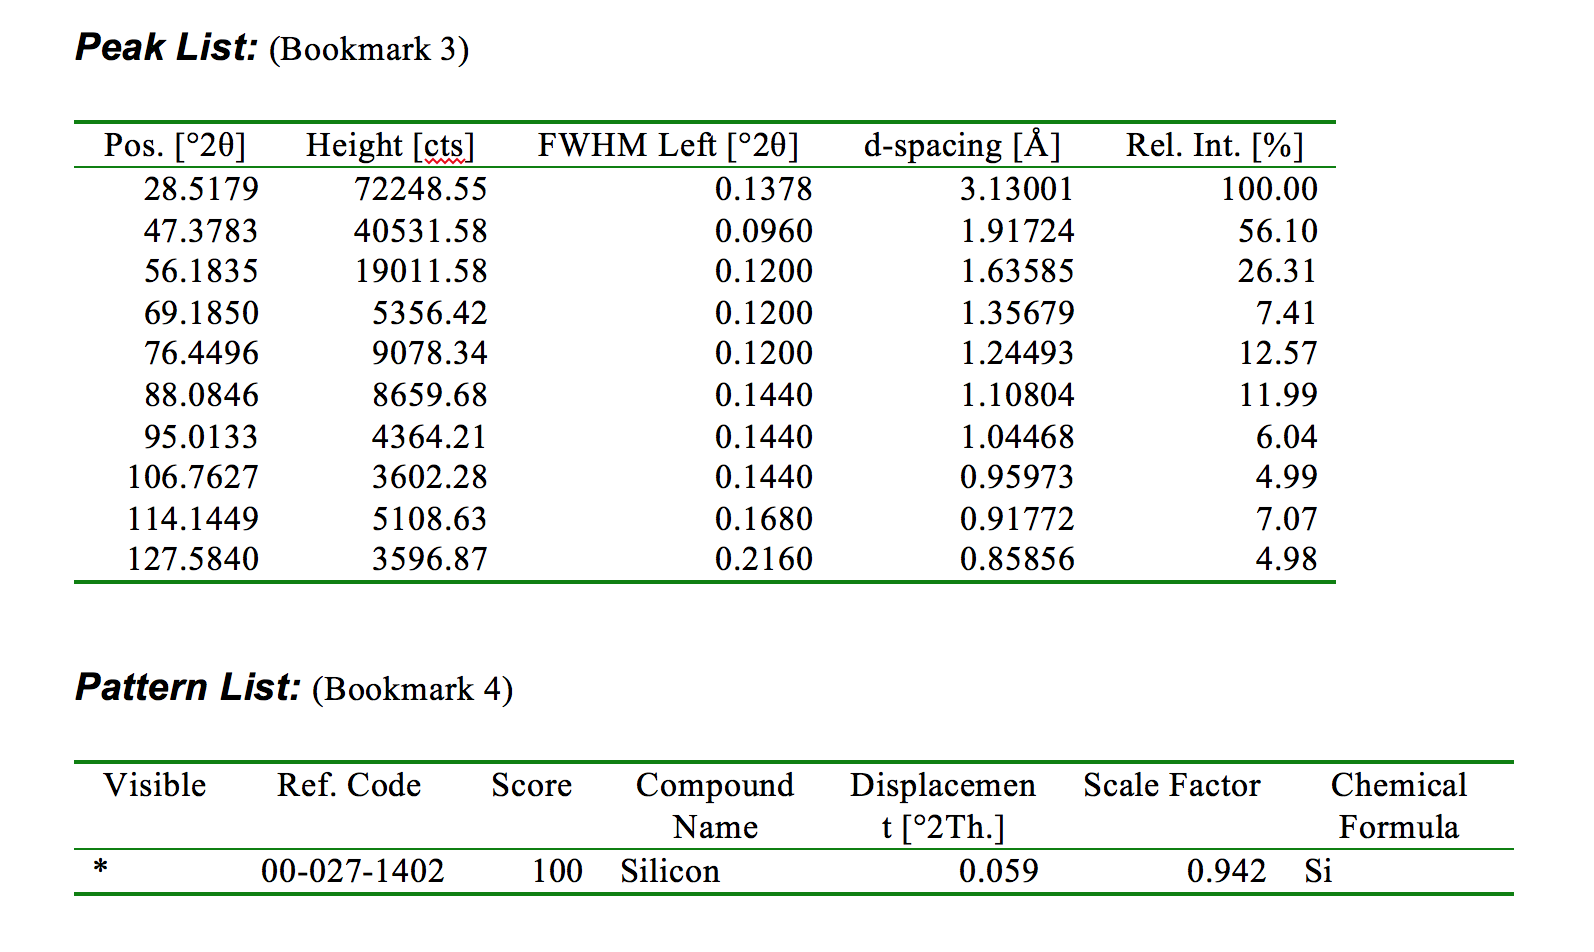
\includegraphics[width=0.65\textwidth]{peaklist} % Include the image peaklist.png
\caption{X'Pert HighScore also provides a peak list in the report}
\end{center}
\end{figure}

%----------------------------------------------------------------------------------------
%	SECTION 5
%----------------------------------------------------------------------------------------

\section{Discussion}
Some considerations can help the use of X'Pert HighScore: choosing single phase over multi-phase, for instance, can influence the match automatically chosen by the software and thus the scores of each candidate for a match.  


%----------------------------------------------------------------------------------------
%	SECTION 6
%----------------------------------------------------------------------------------------

\section{Answers to Multiple Choice Questions}
\begin{enumerate}[label=(\arabic*)]
\begin{item}
What information can you get from an ICDD file?
d (Lattice parameters, crystal structure, and space group)
\end{item}
\begin{item}
When using X'Pert HighScore to analyze a sample, what feature is generally used in choosing a match?
The search peaks feature, and the Analyze tool set. The program gives a candidate score, which we then use to choose a match. 
\end{item}
\begin{item}
Why do we allow a pattern shift during a search match?
Some x-ray diffraction machines are calibrated slightly differently than others, so a pattern shift allows for the absolute position of the peaks to change but their relative positions remain fixed. 
\end{item}
\begin{item}
When you accept a pattern from the candidate list what happens to the rest of the candidates on the list?
If you drag a candidate from the list up to the accepted area, that candidate's score is now higher and the rest of the candidates on the list get a lower score. 
\end{item}
\begin{item}
If a pattern is automatically identified, is it guaranteed to be correct? 
No, especially if you have chosen the wrong phase or you have a complicated sample.
\end{item}
\begin{item}
What parameters can be changed to change the score of the candidates?
 Dragging a candidate up to accepted or deleting it from the list, possibly identifying the sample as a different phase. 
\end{item}
\end{enumerate}

%----------------------------------------------------------------------------------------
%	BIBLIOGRAPHY
%----------------------------------------------------------------------------------------

\bibliographystyle{apalike}

\bibliography{sample}

%----------------------------------------------------------------------------------------


\end{document}